\documentclass[class=article, crop=false, dvipdfmx, fleqn]{standalone}
\title{航空機設計法第一 \\
レポート課題3 \ 機体三面図(初期案)}
\author{学籍番号 03-170313 飯山 敬大\\
        }
\date{\today}

% packages and libraries
\usepackage[utf8]{inputenc}				%fonts
\usepackage[ipaex]{pxchfon}
\usepackage{pifont}
\usepackage{mathtools, amssymb, mathrsfs, bbm,nccmath}	%math
\usepackage{siunitx, physics}
\usepackage[table]{xcolor}				%colors
\usepackage{tabularx}
\usepackage[dvipdfmx]{graphicx}					%figures
\usepackage{subcaption, wrapfig}
\usepackage{tikz}
\usetikzlibrary{calc, patterns, decorations, angles, calendar, backgrounds, shadows, mindmap}
\usepackage{tcolorbox}					%tables
\usepackage{longtable, float, multirow, array, listliketab, enumitem, tabularx}
\usepackage{listings}					%listings
\usepackage{comment}
\usepackage{hyperref}					%URL, link
\usepackage{url}
\usepackage{pxjahyper}
\usepackage{overcite}					%setting of citation
\usepackage{pxrubrica}					%rubi
\usepackage{fancyhdr, lastpage}			%pagelayout
\usepackage{import, grffile}			%file management
\usepackage{standalone}
\usepackage{bm}
\usepackage{empheq}
\usepackage{pdfpages}
\usepackage{multicol}
% set up for siunitx
\sisetup{%
	%detect-family = true,
	detect-inline-family = math,
	detect-weight = true,
	detect-inline-weight = math,
    %input-product = *,
    quotient-mode = fraction,
	fraction-function = \frac,
	inter-unit-product = \ensuremath{\hspace{-1.5pt}\cdot\hspace{-1.5pt}},
	per-mode = symbol,
	product-units = single,
	}

% setting of line skip
\setlength{\lineskiplimit}{6pt}
\setlength{\lineskip}{6pt}

% setting of indent
\setlength{\parindent}{1zw}
\setlength{\mathindent}{5zw}

% change cite form
\renewcommand{\citeform}[1]{[#1]}

% number equations only when they are referred to in the text
\mathtoolsset{showonlyrefs=true}
%\graphicspath{{images/}{../images/}}

% set up for hyperref
\hypersetup{%
	bookmarksnumbered = true,%
	hidelinks,%
	colorlinks = true,%
	linkcolor = black,%
	urlcolor = cyan,%
	citecolor = black,%
	filecolor = magenta,%
	setpagesize = false,%
	}

\pdfstringdefDisableCommands{%
\renewcommand*{\bm}[1]{#1}%
% any other necessary redefinitions
}
% Include \subsubsection in ToC
\setcounter{tocdepth}{3}

% tabularx
\newcolumntype{C}{>{\centering\arraybackslash}X} %セル内で中央揃え
\newcolumntype{R}{>{\raggedright\arraybackslash}X} %セル内で右揃え
\newcolumntype{L}{>{\raggedleft\arraybackslash}X}

\begin{document}
\section{主翼の設計}
BWB機の設計において, 胴体の設計を行う前に, 主翼の設計を行う必要があると判断したので,
先に主翼の設計を行う.
\subsection{翼型の選定}
遷音速機であるから, 抵抗発散を遅らせるため, スーパークリティカル翼型を採用する.

\subsection{アスペクト比AR, 後退角$\Lambda$, テーパー比$\lambda$, 上端角$\Gamma$}
アスペクト比はレポート問題2より,
\begin{equation}
  AR = 9.0
\end{equation}
とする.後退角$\Lambda$, テーパー比$\lambda$, 上端角$\Gamma$は, 教科書の目安の数字より,
\begin{align}
  \Lambda &= 30[deg] \\
  \lambda &= 0.3 \\
  \Gamma &= 6.0[deg]
\end{align}
と設定した.

\subsection{翼端部,翼根部のコード長}
レポート問題2より,
\begin{equation}
  S = 4939[ft^2]
\end{equation}
であるから,翼幅bは,
\begin{equation}
  b = \sqrt{S \times AR} = 265[ft]
\end{equation}
となる. したがって, 翼端部, 翼根部のコード長は
\[
\begin{cases}
  c_{r} = \frac{2}{1 + \lambda}\sqrt{\frac{S}{AR}} = 45.3[ft] \\
  c_{t} = \frac{2}{1 + \frac{1}{\lambda}}\sqrt{\frac{S}{AR}} = 13.6[ft]
\end{cases}
\]
さらに平均空力翼弦$\overline{c_H}$は,
\begin{equation}
  \overline{c_H} = \frac{2}{3} \overline{c_H}
  \frac{1 + \lambda_H +\lambda_H^2}{1 + \lambda_H}
  = 32.3[ft]
\end{equation}
となる.

\subsection{その他パラメタ}
教科書を参考にし,厚み比$t_r$,揚力傾斜$C_{L_{\alpha}}$はそれぞれ,
\begin{equation}
  t_{root} = 18[\%] , \quad t_{tip} = 12.0[\%], \quad C_{L\alpha} = 4~5[/rad]
\end{equation}
と設定する.また巡航時揚力係数$C_{L_{cruise}}$は
\begin{align}
  C_{L_{cruise}} &= \frac{W_{TO} - 0.4W_F}{qS} \\
  &= \frac{896000 - 0.4 \times 238044}{194 \times 4939} \\
  &= 0.53
\end{align}
となるので,胴体取り付け角$\alpha_i$は,
\begin{equation}
  \alpha _i = \frac{C_{L_{cruise}}}{C_{L_{\alpha}}} = 6.06 [deg]
\end{equation}
となる.

\subsection{BWB機の主翼形状について}
BWB機において後に胴体の設計を行う際に, 翼根でのコード長がこの値では足りないので, 下図のように
翼根でのコード長を延長し,下図のような翼形状とした. この際に, 主翼面積を変更する必要があるとも考えられるが, このレポート
では新しく付け足した部分は一種のキンクとして扱い, 基準翼面積は下図の斜線部分として定義し,
主翼濡れ面積にはこのキンク部を含めて扱うことにする.
\begin{figure}[H]
  \begin{center}
  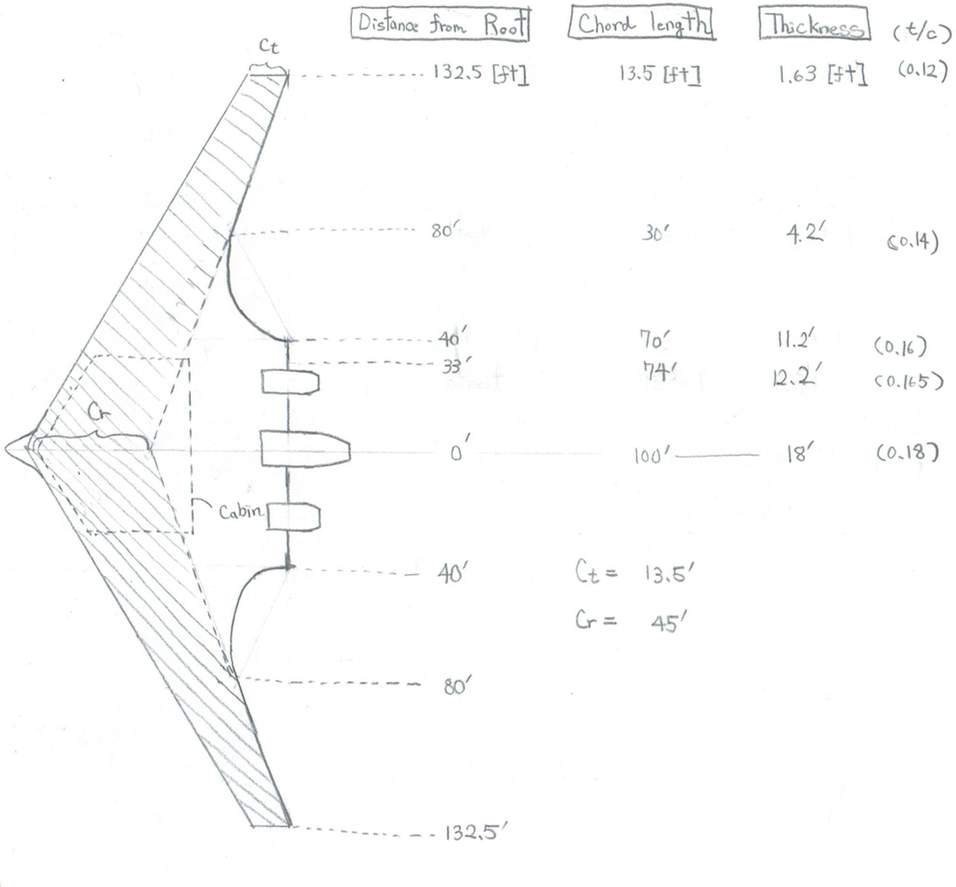
\includegraphics[width=12cm]{../images/wing.png}
  \caption{主翼}
  \label{fig::wing}
\end{center}
\end{figure}

\subsection{燃料タンク容量$V_t$}
教科書記載の統計式より,燃料タンク容量$V_t$は,
\begin{equation}
  V_t = 0.54\frac{S^2}{b}t_{root}\frac{1+\lambda \sqrt{\frac{t_{tip}}{t_{root}}} +
  \lambda^2 \frac{t_{tip}}{t_{root}}}{1 + \lambda^2}
  = 8091[ft^3] = 60527[gal]
\end{equation}
必要な燃料体積$V_F$は,
\begin{equation}
  V_F = \frac{W_F}{\rho_F} = \frac{238044[Ib]}{6.7[Ib/gal]} = 35528[gal]
\end{equation}
$V_F < V_t$より, 十分である. \\
BWB機なので, 翼の内部には客室が配置されるが, 前述した通り, キンク部の存在により, 実際にはより多くのスペースを確保できるので, 十分であると
みなせる.




\end{document}
